\documentclass[12pt]{article}
\usepackage[T1]{fontenc}
\usepackage[margin=1in]{geometry}
\usepackage{amsmath,amssymb}
\usepackage{graphicx}
% A clone receives no PNG under paper/ (the .gitignore paper/** rule), so the
% bare \includegraphics names below resolve only for someone who already holds
% the untracked copies. These are the tracked originals: figures/ carries the
% twelve generated figures, and the Monte Carlo panel belongs to the fold-in
% production run (abm/monte_carlo_trapped_liquidity.png is the Berger run and is
% NOT the panel this manuscript prints).
\graphicspath{{./}{../../figures/}{../../abm/data/runs/run-2026-07-04-15yr-foldin/}}
\usepackage{float}
\usepackage{array}
\usepackage{longtable}
\usepackage{booktabs}
\usepackage{threeparttable}
\usepackage{caption}
\usepackage{authblk}
\usepackage[authoryear,round]{natbib}
\usepackage{xurl}
\usepackage[hidelinks]{hyperref}
\usepackage{microtype}
\emergencystretch=1.5em
\renewcommand{\thesection}{\Roman{section}}
\renewcommand{\thesubsection}{\thesection.\Alph{subsection}}
% Possessive citation: one macro so a bibliography change cannot desynchronize
% hand-rolled \citeauthor{X}'s (\citeyear{X}) constructions.
\newcommand{\citepos}[1]{\citeauthor{#1}'s (\citeyear{#1})}

\title{Mortgage Lock-In and the Federal Reserve's Quantitative Tightening Shortfall}
\author{Eugene Ong}
\affil{Carnegie Mellon University}
\date{}
\begin{document}
\maketitle
\begin{abstract}
\noindent U.S. agency mortgage-backed securities buy To-Be-Announced market liquidity with pool homogeneity built from standardized fixed-rate contracts whose par-payoff obligation, enforced through due-on-sale, locks households into below-market coupons when rates rise. This paper measures that trade-off's cost to the Federal Reserve during Quantitative Tightening, when agency MBS runoff fell \$764.7 billion short of the phased redemption caps over June 2022--November 2025. It cost less than the shortfall suggests. A loan-level survival framework built from Freddie Mac performance data recovers 91.3\% of that shortfall on a benchmark-consistent accounting basis at the headline off-window calibration, 88.2--93.7\% across that calibration's defensible range; at the in-sample calibration point on which the framework was assembled it recovers 97.9\%. Under the production hard-maximum form a null without the lock-in elasticity still recovers 85.7\% at the headline calibration (88.7\% in-sample; 35.6\% under the additive form), because scheduled amortization plus a turnover floor undershoot a \$35 billion monthly cap under any household response to rates. The Federal Reserve's own ex-ante projection anticipated the large majority of the realized shortfall. Measured against that projection rather than the never-binding cap, lock-in accounts for roughly a quarter to a half of the genuine surprise, depending on a disclosed intra-2022 allocation choice: the settlement-aware allocation matching the realized settlement pattern gives the quarter, the pre-committed uniform-spread central allocation the half. The design identifies a bounded range for the elasticity's contribution, not a pinned magnitude, and it identifies neither a level nor monthly timing: no monthly-timing claim survives its own placebo tests, and the margin's sign is fixed by a rate configuration that leaves essentially the whole book out of the money throughout the window, not by the estimated elasticity. Re-anchoring the baseline turnover floor that dominates the level outside the evaluation window and off the locked-in population puts that contribution at $+5.6$ percentage points over the rate-inelastic baseline ($+\$42.6$ billion), $+4.3$ to $+6.8$ points across the off-window floor's defensible range under the production hard-maximum form ($+3.0$ to $+8.0$ once the floor reads' cluster-bootstrap sampling error is propagated, open below $+4.3$ on an age-standardized read; wild-cluster correction of that read's under-coverage gives $+2.9$ to $+8.7$, the widest uncertainty source with a coverage property though not the widest read of that source, while the unestimated baseline seasoning ramp spans $+0.9$ to $+15.6$ at the same calibration); under the disclosed additive form the same anchors return $+11.2$ points nearly floor-invariantly, so the form-conditional identified range is $+3.5$ to $+13.1$ points, with $+5.6$ its max-form member; the in-window production calibration returns $+9.2$ points, which I now report as an in-sample calibration point, not the headline. The margin is positive at every floor and elasticity-band combination tested (a specification check the rate configuration cannot let fail, retained as such), and its magnitude is unchanged under a floor calibrated only on the window's first nineteen months, an input-stability check rather than an outcome holdout: no outcome-holdout months exist anywhere in this design. An agent-based model of the moving decision recovers 13.6\% averaged across seeds, though a cross-design variant recalibrated on real loan covariates recovers 59.3\% on the frozen seed and 60.2\% averaged over fifty seeds (76.3\% reweighted to the book's composition). The contrast cannot be cleanly attributed to modeling paradigm. The mobility cost is real. The institutional cash-flow cost is small; its sign turns on the transplant's anchor, not on any within-anchor sensitivity sweep: importing Denmark's baseline mobility along with its payoff rule yields roughly $-\$100$ billion, while a transplant changing only the payoff rule yields $+\$61$ billion at the in-sample calibration point and $+\$28$ billion at the off-window calibration the headline marginal uses. The latter's positivity follows from anchoring the Danish leg at the U.S. zero-gap hazard on a book out of the money almost everywhere; the informative quantity there is the magnitude, not the sign.
\end{abstract}

\vspace{0.5\baselineskip}
{\footnotesize\noindent\textbf{Keywords:} mortgage prepayment; lock-in effect; quantitative tightening; mortgage-backed securities; hazard models; monetary policy implementation.\\
\textbf{JEL codes:} E52, E58, G21, R31.\par}
\newpage
\section{Introduction}\label{sec:intro}
The Federal Reserve allowed agency mortgage-backed securities (MBS) to run off
passively when Quantitative Tightening began in June 2022, subject to a cap that
rose from \$17.5 billion to \$35 billion per month. Principal payments never
reached the full cap. Through November 2025, realized runoff was \$764.7 billion
below the phased ceiling. This paper asks how much of that shortfall reflects
mortgage-rate lock-in rather than scheduled amortization and turnover that would
have occurred even without a rate response.

The distinction matters because a cap is a ceiling, not a forecast. The New York
Fed's May 2022 baseline already implied that 75.6--88.5\% of the eventual
cap-relative shortfall would occur, depending on how its annual 2022 projection
is allocated within the year. I therefore report both the policy-committed
\$764.7 billion benchmark and an expectations-based complement. The latter is
\$87.8 billion, but it may already embed part of the lock-in channel and the
spring-2022 expected rate path differed from the realized one. Ratios stated
against it are consequently upper bounds on lock-in's share of a mixed
lock-in-and-rate-path surprise.

The primary estimate is a loan-level hazard microsimulation on Freddie Mac
loans. Its rate-inelastic null switches off the imported rate-gap elasticity
while retaining scheduled amortization, seasoning, burnout, observed borrower
covariates, and a turnover floor measured from realized deep-discount cohorts.
At the off-window floor used for the headline, that null recovers 85.7\% of the
cap-relative benchmark under the production maximum-floor form; the central
simulation recovers 91.3\%. Their difference is the paper's identified object.
Propagating sampling error in the off-window floor with the pre-committed
wild-cluster procedure gives a binding interval of $+1.9$ to $+9.1$ percentage
points. The $+5.6$-point, \$42.6 billion mid-grid value lies inside that range
but is an anchor convention, not the estimate the design identifies. At the
in-window calibration point the difference is $+9.2$ points, reported as an
in-sample comparison.

This is an accounting decomposition within a disclosed model, not causal
identification. The elasticity is imported from estimates of how mortgage-rate
gaps change mobility; it is not re-estimated here. The turnover floor contains
discretionary and involuntary moves and therefore is not a non-behavioral
baseline. Functional form matters: an additive competing-risks specification
changes the aggregate level and produces a form-conditional marginal hull of
$+3.5$ to $+13.1$ points. The result is thus a bounded marginal over a
rate-inelastic null, not a claim that lock-in caused the entire runoff
shortfall.

Two validation exercises limit the interpretation. A household-choice
agent-based model recovers only 13.6\% on its synthetic population, but rises
above a pre-committed threshold when run on real structural covariates; the
paper therefore withdraws the claim that the cross-model
difference identifies a modeling-paradigm effect. A Fannie Mae reproduction
returns a similar marginal, but it is a robustness check, not an outside test:
both agencies share the same policy window and the same transported elasticity.

The policy implication is narrower than the accounting shortfall. Scheduled
amortization and baseline turnover were already too small for a \$35 billion
monthly MBS cap to bind in almost every month, so the cap was set above
achievable passive runoff under the modeled book. A Danish-style
market-value-repurchase rule illustrates how contract design could change the
cash-flow channel. The rule-only U.S.-intercept transplant produces a
+\$61.2 billion face-value gap at its zero-refinance edge, while a
Danish-level anchor reverses the sign to -\$99.9 billion and cash accounting
can reverse it again. The counterfactual is therefore anchor- and
incidence-dependent and does not price the TBA liquidity cost of redesigning
U.S. agency securitization.

The paper contributes the cap-relative and expectations-based benchmarks, the
hazard decomposition with its binding uncertainty, and the ex-ante cap-design
arithmetic. The ABM comparison and Danish exercise are validation and policy
counterfactuals, not additional headline estimates. The technical and
replication supplement preserves the full specification, diagnostic grids,
adjudications, and run history omitted from the publication-facing argument.

\section{Literature Review}\label{sec:lit}

Mortgage prepayment research moves from frictionless refinancing toward hazards
that combine financial incentives, seasoning, borrower heterogeneity, and pool
selection. Early valuation models treat refinancing as optimal exercise
\citep{dunn1981}; later work adds transaction costs and empirical prepayment
functions \citep{schwartz1989,richard1989,stanton1995,agarwal2013}. This paper
uses that second tradition. Its rate-inelastic null is scheduled amortization
plus a measured turnover floor, while the central leg adds a transported
rate-gap response. Burnout enters through loan-level survival rather than a
representative borrower, consistent with selection in heterogeneous pools
\citep{chernov2018,lesniewski2026}.

Recent evidence establishes that the 2022 rate increase reduced refinancing and
mobility. \citet{batzer2024} estimate large amounts of retained below-market
financing value and foregone moves. \citet{liebersohn2024} estimate that each
percentage point by which market rates exceed a borrower's coupon reduces
quarterly mobility by 5.5--7.7\%, the calibration band used here.
\citet{graybill2026} obtain a somewhat larger sale-hazard response from
transaction data. \citet{aladangady2024} find that rate-gap lock-in explains
44\% of the observed decline in borrower mobility, leaving substantial room
for other housing and behavioral channels. These studies identify or calibrate
the household response. This paper instead asks how much that response adds to
the Federal Reserve's MBS cash-flow shortfall after rate-insensitive turnover
and amortization are held fixed.

Federal Reserve staff already document the institutional fact. \citet{na2024}
report that most SOMA MBS were far out of the money to refinance, that principal
payments remained below the cap, and that realized payments were composed
roughly of scheduled principal and turnover-related prepayment. Staff and
official accounts likewise describe persistent below-cap runoff
\citep{nyfed2022,perli2024,hammack2025}. Their result concerns the composition
of realized payments. The null in this paper asks a different question: how
much of the shortfall against the cap is reproduced by those rate-insensitive
components? Extending the measurement through November 2025 and comparing the
central and null simulations produces the marginal reported here.

The paper also relates to evidence that mortgage refinancing transmits monetary
policy and changes the duration supplied to investors
\citep{dimaggio2020,berger2021,eichenbaum2022,krishnamurthy2011,vayanos2021}.
The tightening episode reverses the familiar easing channel: a stock of
low-coupon mortgages created during the refinancing boom becomes long-lived
when rates rise. That duration matters for banks and MBS investors
\citep{jiang2023,malkhozov2016}, but this paper measures portfolio cash flow,
not the general-equilibrium price of duration risk.

Finally, the Danish mortgage system supplies the institutional counterfactual.
Its balance principle and market-value-repurchase option allow a borrower to
retire debt by purchasing and delivering the corresponding bonds
\citep{berg2018,frankel2004,svenstrup2006}. \citet{berger2026} estimate a
near-flat Danish mobility response to the coupon gap. Their slope estimate does
not provide the level of U.S. mobility under Danish rules, so the
counterfactual reports both a U.S.-intercept rule-only transplant and a
Danish-level bracketing anchor. The difference between them is part of the
result, not a nuisance to be averaged away.

\section{Empirical Methodology}\label{sec:method}

\subsection{Two Structurally Distinct Estimators of the Aggregate Level}\label{sec:method-estimators}

The first estimator is a 10,000-household Agent-Based Model (ABM), specified in Appendix~\ref{sec:method-abm}. It draws a synthetic population calibrated to aggregate FRED medians. It then tests whether a utility-maximizing household decision rule, rational or behaviorally extended, can account for the shortfall; Section~\ref{sec:abm} reports its results. The second is a hazard framework, specified in Section~\ref{sec:hazard}. It abandons the household utility function entirely and models loan-level survival directly on real Freddie Mac loan-level data. It runs along two paths. Path A is a stratum-month discrete-time hazard model, estimated by Poisson pseudo-maximum likelihood on the full 2017--2021 origination universe aggregated to stratum-months. Path B is a loan-level microsimulation with competing prepayment and default risks, run on a stratified 75,000-loan sample drawn from that universe.

I evaluate both estimators against the same \$764.7 billion empirical benchmark (Section~\ref{sec:method-benchmark}) and the same June 2022--November 2025 QT window. Their results are therefore directly comparable, even though they draw on different data and different behavioral assumptions. They differ in modeling paradigm (household choice versus loan-level survival) and, on the hazard side, in the use of real loan-level data. Population size differs too: 10,000 households against Path B's 75,000 simulated loans, with Path A estimated on the full origination universe. Section~\ref{sec:robustness} finds that this size difference does not drive the gap in their explanatory power. The data-source difference, though, remains an unresolved confound. It is why the ABM--hazard contrast cannot be cleanly attributed to modeling paradigm rather than to calibration and data source, the reading Section~\ref{sec:robustness-crossdesign} withdraws on a pre-committed threshold crossing. Figure~\ref{fig:architecture} maps the pipeline.

\begin{figure}[H]
\centering
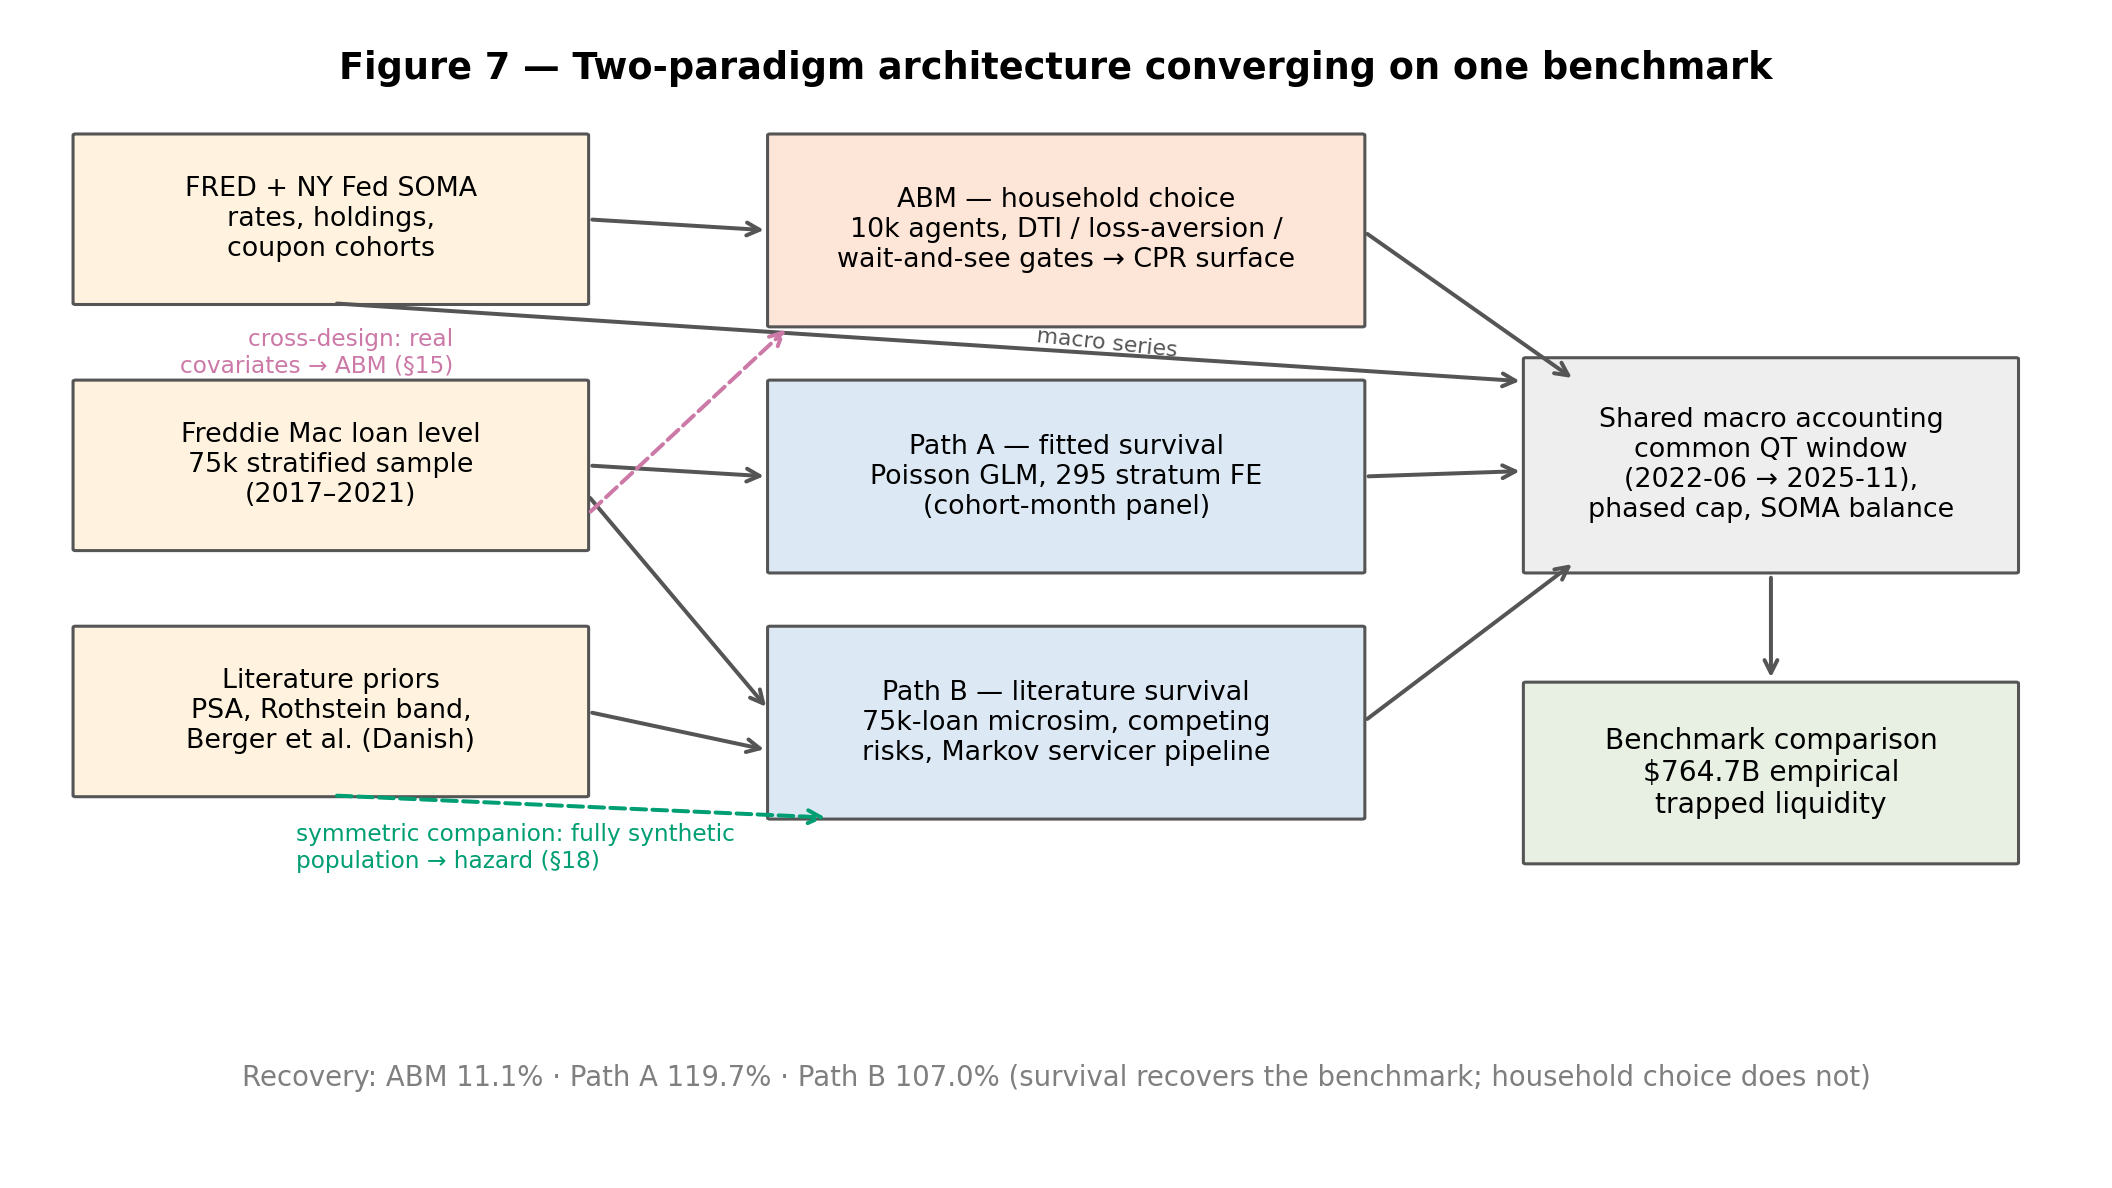
\includegraphics[width=\textwidth]{fig7_architecture}
\caption{Pipeline architecture. Data sources (FRED macro series, NY Fed SOMA holdings, Freddie Mac loan-level performance) feed three estimators (the synthetic-population ABM and hazard Paths A and B), whose simulated roll-off paths are scored through one shared macro-accounting layer against the \$764.7 billion empirical benchmark of Section~\ref{sec:method-benchmark}. The two robustness cross-links are the cross-design test (real Freddie covariates into the ABM, Section~\ref{sec:robustness-crossdesign}) and the symmetric companion test (synthetic population into the hazard framework, Section~\ref{sec:robustness-synthesis}).}
\label{fig:architecture}
\end{figure}

The agent-based model's specification and the structural extensions used by Section~\ref{sec:abm} are summarized in Appendix~\ref{sec:method-abm} and documented fully in the technical replication supplement.

\subsection{Empirical Validation Benchmark}\label{sec:method-benchmark}

I build the empirical shortfall benchmark from the New York Fed's SOMA current face value series. It nets realized roll-off against the actual phased redemption caps (\$17.5 billion per month June--August 2022, \$35 billion per month from September 2022), strictly within the active QT window, June 2022--November 2025. Accumulation is net rather than shortfall-months-only, for comparability with the Danish counterfactual of Section~\ref{sec:abm-danish}, whose simulated roll-off routinely exceeds the cap. The terminal gaps in Figure~\ref{fig:benchmark} are the cap-relative benchmark and the expectations-based complement below. One feature of the series is an artifact: four months come in at exactly zero. No result in this paper reads it as behavior. The cause is the back-out's non-negativity clip. It pins any month whose reported roll-off falls below scheduled amortization and displaces the mass into the next month, a month-boundary allocation artifact of the reporting series (run \texttt{h1\_zero\_months\_diagnosis}). Appendix~\ref{sec:robustness-seasonalfloor} traces the mechanism and shows that repairing the affected pairs flips this paper's frozen monthly-timing rule from pass to concede. That artifact is one reason every claim made from this benchmark is a claim about levels.

\begin{figure}[H]
\centering
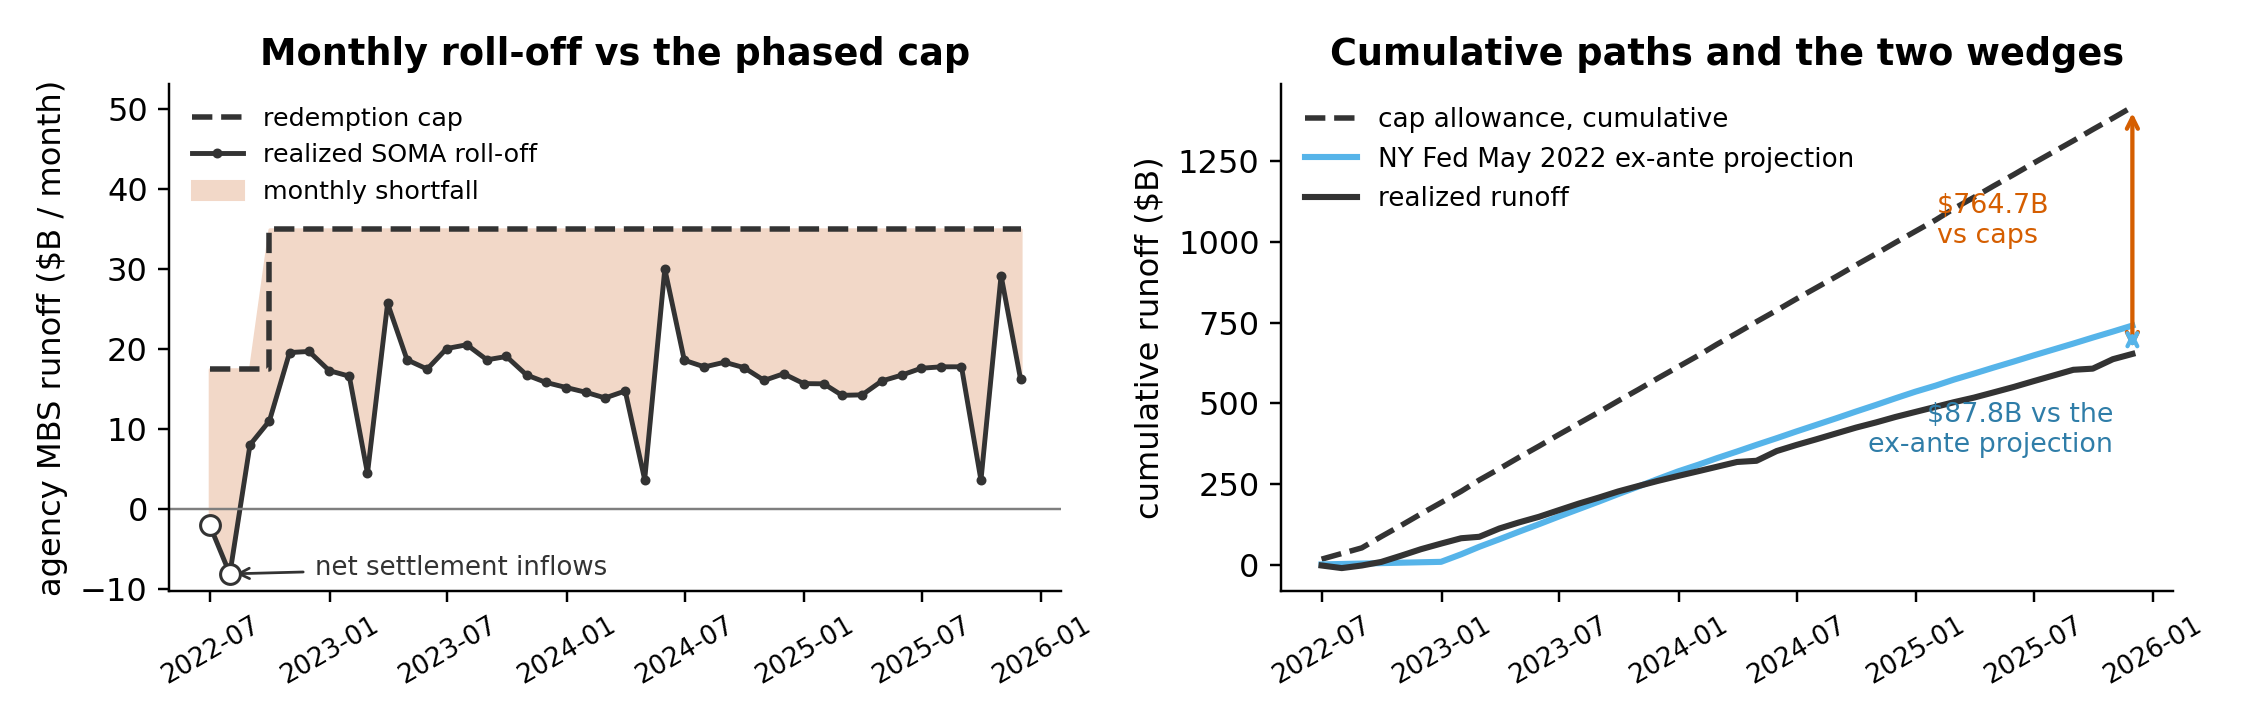
\includegraphics[width=0.94\textwidth]{fig9_benchmark_construction}
\caption{The empirical benchmark. Left: realized monthly SOMA agency MBS roll-off against the phased redemption cap; the shaded area is the monthly shortfall, which accrues on a net basis (the two circled opening months are net settlement inflows). Right: the same construction cumulatively. The terminal gaps are the \$764.7 billion cap-relative benchmark and, against the New York Fed's May 2022 ex-ante projection, the \$87.8 billion expectations-based complement. Monthly series from the frozen production run's metrics; the projection's monthly path is derived from the published year-end levels under the pre-committed uniform-spread rule and asserted, in the generator, to reproduce the frozen expectations-run totals.}
\label{fig:benchmark}
\end{figure}

\begin{table}[H]
\centering
\small
\caption{Headline quantities on the benchmark-consistent accounting basis.}
\label{tab:headline-compact}
\begin{threeparttable}
\begin{tabular}{@{}p{5.2cm}p{3.0cm}p{5.5cm}@{}}
\toprule
Object & Result & Interpretation \\
\midrule
Cap-relative benchmark & \$764.7 billion & Accounting shortfall against the phased ceiling; not a causal estimate \\
Production ABM & 13.6\% & Fifty-seed mean on its synthetic population; 10--17\% seed band \\
Path B central, off-window floor & 91.3\% & Loan-level hazard level with the transported rate response active \\
Rate-inelastic null, $\beta_1=0$ & 85.7\% & Scheduled amortization, measured turnover floor, seasoning, burnout, and covariates retained \\
Lock-in marginal, off-window floor & $+5.6$ pp; $+\$42.6$ billion & Central minus null at the mid-grid anchor; the binding result is $[+1.9,+9.1]$ pp \\
\bottomrule
\end{tabular}
\begin{tablenotes}[flushleft]\footnotesize
\item Notes: Recovery percentages divide by the unrounded \$764.748 billion benchmark. The ABM is a stress test and is not averaged with Path~B. The Path~B level is not the lock-in effect: the publication-facing result is the marginal over the rate-inelastic null. The off-window anchor uses the 4.991\% floor read and the adopted 6.5\% mobility-response calibration.
\end{tablenotes}
\end{threeparttable}
\end{table}

The empirical shortfall is approximately \$764.7 billion (unrounded: \$764.748 billion; every percentage-of-benchmark figure in this paper divides by this value). It is the benchmark for simulated trapped liquidity in Sections~\ref{sec:abm} and~\ref{sec:hazard}. The SOMA face spans the Federal Reserve's full agency MBS book, Ginnie Mae collateral included, 20.4\% of face. Of that face, 66.2\% lies in the 2017--2021 vintages of the Freddie Mac loan-level sample (Section~\ref{sec:hazard}). The hazard framework therefore samples directly neither Ginnie collateral nor roughly one-third of the book by vintage. Section~\ref{sec:pathb} bounds both exclusions externally; Section~\ref{sec:limitations} states what each bound leaves open. The exclusions must be netted on the book's own joint cells, not counted separately. Out-of-window vintage is 33.7\% of face (2022 cohort 23.1\%, pre-2017 10.6\%), and the 20.4\% Ginnie share cuts across vintage. The conventional-and-in-window intersection is therefore 51.0\% on the book's own agency $\times$ vintage joint cells (bounded above by 51.8\% for cell truncation; 52.7\% under an independence approximation). The Freddie 2017--2021 conventional universe estimating Path B is about \emph{half} of SOMA book face. Two-thirds is the vintage-only marginal and overstates coverage. External-speed overlays (Section~\ref{sec:pathb}) bound Ginnie at \$20--\$47 billion by published observed speeds, and out-of-window vintages at \$11.7 billion by observed cohort speeds from the replication ingest. Each bound is signed toward overstating trapped liquidity. On the simulated side an income-scaled curtailment assumption enters, averaging approximately 0.84\% annualized and consistent with GSE daily prepayment report estimates. It is added to each simulated roll-off and netted as a common dollar item in the shared accounting layer of Section~\ref{sec:robustness-hybrid}, so the empirical CPR back-out's series retains that component. Two implementations of the back-out exist: the ABM's cohort-weighted, term-aware scheduled amortization and the hazard side's single-pool approximation. Both amortize at the pass-through WAC, though scheduled principal follows the borrowers' note rate, that WAC plus a $+0.80$-point guarantee-fee and base-servicing wedge. On the note-rate basis the hazard-side CPR level rises $+0.27$ points, a deterministic schedule difference. Every trapped-dollar figure is bit-identical: the benchmark's dollars never pass through the CPR scale. Every peak lag and $U_2$ is unchanged at reporting precision, correlations differing only at the third decimal (run \texttt{coupon\_convention\_amortization}). The corrected-basis timing diagnostics are summarized in Appendix~\ref{app:theil}.

\paragraph{Accounting bases.} Every recovery percentage in this paper is quoted on one of four accounting bases, differing only in two orthogonal choices, pure accounting layers with no modeling content: whether the common curtailment flow is netted out, and whether the estimation sample is reweighted to the SOMA book's coupon mix. The \emph{standalone-scorer basis} makes neither adjustment; the \emph{benchmark-consistent shared basis} nets that common curtailment flow (\$69.56 billion over the window) identically from every U.S. leg, a flat 9.1 percentage points of the benchmark for every U.S. estimator; the \emph{full-book basis} instead reweights the standalone figure to the book's weighted-average coupon (WAC) without netting; and the \emph{composed basis} applies both, the same 9.1-point netting to the full-book figure. Because the netting is bit-identical across central and null legs, it cancels exactly from the lock-in marginal and every cross-estimator gap, an invariance at every cell of the calibration box and under a $\pm 25\%$ stress on the assumed curtailment rate (derivation and stress in Section~\ref{sec:robustness-hybrid}; the accounting bases summarized in Appendix~\ref{app:params}). The cancellation is term-by-term monthly, not merely aggregate: the netted flow is a shared monthly rate times the shared actual-holdings path, so any curtailment time profile (calendar-seasonal, or income elasticities differing across sub-periods) cancels identically, moving only the common wedge. The income-to-rate mapping's functional form is immaterial to the marginal for the same reason: any alternative (concave, threshold, or piecewise in income) yields another shared profile. Main-text headline figures are quoted on the shared basis throughout.

I construct a second, expectations-based benchmark because the cap-relative one carries a tension: the caps were widely expected to be non-binding for agency MBS, so a shortfall measured against them mixes an anticipated rate-inelastic component with genuine surprise. Against the Federal Reserve's own ex-ante projection, projected agency MBS runoff is \$740.6 billion and realized runoff \$652.8 billion: an expectations-based shortfall of \$87.8 billion, 11.5\% of the cap-relative \$764.7 billion. That projection is the baseline path published in the New York Fed's May 2022 Open Market Operations annual report \citep{omo2021}, starting from the February 2022 balance sheet, incorporating the FOMC's May 2022 Plans, and modeling runoff from June 2022. I spread its year-end figures uniformly within each printed year and clip them to the window under a rule fixed before the numbers were seen. The report prints year-end levels only, and no staff projection at monthly granularity is public for any vintage covering this window. Equivalently, that projection already implied 75.6--88.5\% of the realized cap-shortfall, the range spanning defensible intra-2022 allocations of its printed annual net. The pre-committed uniform-spread central construction gives \$676.9 billion, or 88.5\%. The substantive point is that a source predating every estimate in this paper anticipated the large majority of the shortfall, and it stands on its own. A sharper reading it invites does not. Under the uniform-spread construction the 88.5\% sits 0.2 points from the 88.7\% the $\beta_1 = 0$ rate-inelastic null recovers on the benchmark-consistent basis, and I presented that near-equality as convergent evidence. I withdraw the presentation: the 0.2 points require two conditions at once. They require the in-sample 4.0\% turnover floor, because at the off-window floor the paper headlines, the null recovers 85.7\% and falls 2.8 points \emph{below} the projection, not 0.2 above it. And they require the uniform-spread allocation, because the settlement-aware allocation puts the anticipated share at 75.6\%, which the null clears by 13.2 points in-sample and 10.1 points at the headline floor. A $-2.8$ to $+13.2$ point span across two disclosed choices is not a convergence, so I now report the projection range and the null's recovery separately. Both recoveries are production-floor-form reads, so the comparison is against one form's null, not a form-invariant object. Under the additive form the null recovers 35.6\% on the benchmark-consistent basis at the headline floor (44.7\% standalone; Section~\ref{sec:robustness-floor}). What survives is coarse and is what I rely on: under the production floor form both objects put the anticipated rate-inelastic component in the large majority of the shortfall. That is a fact about where the caps were set, not the size of the rate response, since the caps sat above any prepayment path this book could have delivered. Leading with it understates lock-in; the reading that speaks to mortgage markets is the marginal's share of the expectations-based shortfall, below. The central 88.5\% rides on the uniform-spread treatment of the printed 2022 annual net, which nets first-half settlement inflows against June--December runoff. That is the less faithful of the two constructions to the realized settlement record. The settlement-aware allocation assigns those inflows to the first half (realized: holdings rose \$92.3 billion over January--May 2022 in the benchmark's own SOMA series), giving roughly three-quarters (75.6\%). It leaves the large-majority reading, and every gate and threshold of the run, unchanged. Parametric within-year ramps bound the rest. Linear 2022 ramps move the share only to 88.0--89.0\%, the December-2025 window clip spans 86.1--90.6\% between all-front and linear-back extremes, and the bracket pushing all 2025 runoff to the clipped December raises it to 115.3\%. The rate-inelastic-majority threshold survives at every allocation. Every percentage-of-benchmark figure in this paper remains a cap-basis quantity. Dollar objects and estimator rankings are basis-invariant, the decomposition rescaling by the $8.7\times$ benchmark ratio on the expectations basis. The identified lock-in marginal is 49\% of the expectations-based shortfall under the central uniform-spread construction at the headline off-window floor ($+\$42.6$ billion), 80\% at the in-sample calibration point ($+\$70.3$ billion). That shortfall is itself allocation-dependent, so the ratio falls with the anticipated share (roughly 23\% and 38\% at the 75.6\% allocation) and is undefined at the extreme 115.3\% bracket, where the expectations-based shortfall turns negative. Every one of these ratios rests on one condition I cannot test: it reads the expectations-based shortfall as a residual free of lock-in, when the projection's own prepayment model may already have embedded part of the channel. That is unrecoverable from the published path of holdings. Any lock-in the projection anticipated therefore sits inside the \$740.6 billion, not the \$87.8 billion residual, and the ratios are upper bounds on lock-in's share of the genuine surprise, exact only if the projection embedded none of the channel. A second condition is likewise untestable from the published record: the projection conditions on the spring-2022 market-implied rate path, well below what was realized, so part of the residual is rate-path surprise, not lock-in. Both are properties of the projection, not of any one quotation of it, so they govern every site where these ratios appear (introduction, this section, conclusion). Each reads as an allocation-conditional upper bound on lock-in's share of a mixed lock-in-and-rate-path surprise, not a partition of it. One question of standing precedes this accounting: a shortfall against the MBS cap is not by itself evidence that a stated policy objective was missed. The Committee's operating object was the aggregate securities portfolio's decline, Treasury runoff ran against its own caps throughout, and nothing in this paper shows that reserves or the aggregate path came in off the intended course because MBS ran slow. The \$764.7 billion measures the \emph{composition} of the decline (MBS principal that did not arrive on the book's own schedule) and the duration consequences it carries (Section~\ref{sec:discussion-fallout}): how the decline was delivered and what that cost in portfolio structure, not a claim that the decline itself fell short.

The benchmark measures shortfall against the redemption cap, a ceiling on runoff. The cap is not a forecast. New York Fed staff projected the below-cap regime from the month the \$35 billion cap took effect \citep{nyfed2022}. The cap-relative shortfall is therefore an upper bound on the shortfall relative to any reasonable ex ante expectation. The complement above quantifies it: the expectations-based shortfall is \$87.8 billion, 11.5\% of the cap-relative figure. I retain the cap as the headline counterfactual for two reasons. First, it is the only policy-committed quantity available. The projection underlying the complement is a baseline forecast, not an FOMC-stated target. Adopting any forecast, the Federal Reserve's or a model's, would be circular with respect to models of expected prepayment, the object under study. Second, it is policy-relevant: it measures the gap between the maximum balance-sheet reduction the FOMC authorized and the reduction the mortgage structure delivered. ``Trapped liquidity'' and ``shortfall'' accordingly denote the shortfall relative to the cap throughout the paper.
\section{Agent-Based Model: A Stress Test}\label{sec:abm}\label{sec:abm-results}
The agent-based model (ABM) is a cross-design stress test, not the paper's
primary estimate. It applies a household move/stay rule to 10,000 synthetic
households and aggregates those decisions into MBS cash flows. The
fifty-seed production mean recovers \$103.7 billion, or 13.6\% of the
cap-relative benchmark; the frozen seed-42 draw recovers 11.9\%. Seed
dispersion puts the useful reading at roughly 10--17\%, rather than at a
three-digit point estimate. The model also misses the monthly path: simulated
mean CPR is 11.68\% against an empirical 5.14\%, lag-0 correlation is
$-0.318$, and $R^2$ against a mean-only null is $-6.984$. Behavioral
extensions and the fifteen-year fold-in do not repair that mismatch. A burnout
variant collapses simulated prepayment because its closed population exhausts
mobile households before QT; it is an adverse falsification, not a production
result.

\begin{figure}[tbp]
\centering
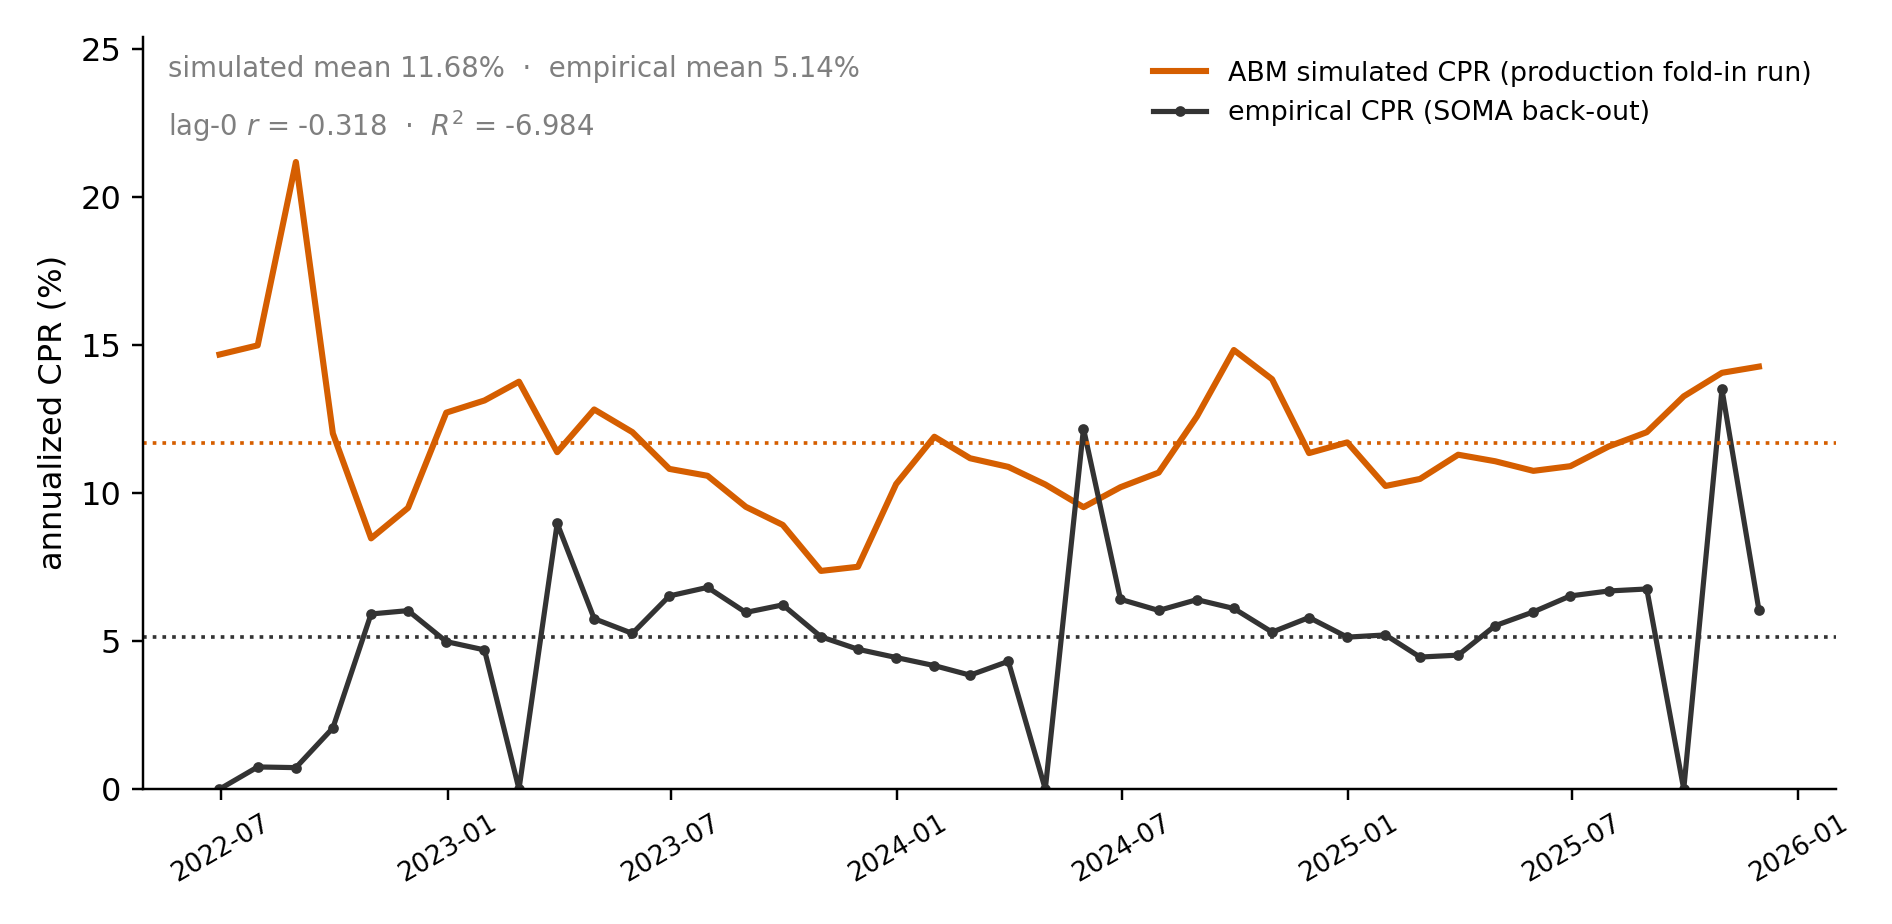
\includegraphics[width=0.86\textwidth]{fig10_abm_cpr_paths}
\caption{Production ABM CPR against the SOMA-implied benchmark over the QT
window. The model overpredicts the level and does not track the monthly shape;
the comparison is a diagnostic rather than validation of the ABM estimate.}
\label{fig:abmpaths}
\end{figure}

The model's low recovery cannot be attributed cleanly to modeling paradigm.
Replacing its synthetic structural covariates with Freddie Mac covariates raises
recovery to 59.3\% on the committed draw and 60.2\% over fifty seeds, above the
pre-committed 50\% threshold at which the paradigm interpretation was to be
withdrawn. Reweighting that leg to the SOMA coupon distribution raises it to
76.3\%. The frozen-calibration leg moves in the opposite direction under the
same reweighting, and the borrower-behavior variables remain synthetic in every
case. The result therefore identifies sensitivity to population and calibration,
not a clean comparison between agent-based and hazard modeling.

Nor does the ABM supply a usable lock-in marginal. Its turnover floor is an
outcome of the calibrated move rule rather than a separable component. Holding
the production mobility scale fixed while removing the rate penalty eliminates
the floor and over-retires the book; re-estimating the scale under the null
fits away the differential. The two constructions imply marginals with opposite
signs. I therefore report no ABM marginal and use its level only as a
cross-design robustness check. The full decision rule, population construction,
behavioral extensions, seed results, and null-feasibility probe are preserved
in the technical and replication supplement.

\section{The Hazard Framework: A Structurally Distinct Estimator}\label{sec:hazard}
\subsection{Estimand and specification}\label{sec:hazard-motivation}\label{sec:pathb}\label{eq:pathB}\label{eq:beta1}\label{eq:default}\label{tab:estimators}

The primary design separates the aggregate level recovered by a loan-level
prepayment model from the increment associated with the mortgage-rate gap.
Path~B simulates 75,000 loans drawn from the Freddie Mac 2017--2021 origination
universe. The annualized prepayment hazard combines a baseline turnover floor
with a rate-responsive component, seasoning, burnout, and observed covariates.
Default is a competing exit. Scheduled amortization is calculated from each
loan's note rate, balance, age, and remaining term, and the resulting cash flows
are mapped to the SOMA book.

The rate-gap response is calibrated rather than estimated in this sample.
\citet{liebersohn2024} provide the 5.5--7.7\% mobility-response band; I use
6.5\% as the central specification. Applying a mobility elasticity to total
prepayment assumes that the response transports from moves to the combined move
and refinance hazard. Termination-reason fields do not identify that mapping in
the data used here, so a moving-share mixture is reported as a sensitivity, not
an estimate. The response is also transported across vintages, agencies, and
the QT rate environment.

The baseline floor is measured from deeply out-of-the-money cohorts. It includes
discretionary moves, cash-out refinancing, and involuntary turnover; it is not a
non-behavioral object. The production specification uses a hard maximum between
the fitted hazard and that floor. An additive competing-risks form is reported
because the maximum censors the rate response whenever the floor binds. The
level is consequently floor- and form-dependent.

\subsection{The marginal over the null}\label{sec:identification}

The central simulation recovers 91.3\% of the \$764.7 billion cap-relative
benchmark at the headline off-window floor on the benchmark-consistent basis.
The $\beta_1=0$ null removes only the imported rate-gap response and retains
scheduled amortization, baseline turnover, seasoning, burnout, covariates, and
the common accounting layer. It recovers 85.7\%. Their difference is the
lock-in marginal:
\begin{equation}\label{eq:marginal}
\Delta^{LI}=R(\widehat\beta_1,\widehat h_0)-R(0,\widehat h_0).
\end{equation}
At the off-window mid-grid anchor, $\Delta^{LI}=+5.6$ percentage points, or
\$42.6 billion. At the in-window 4\% floor it is $+9.2$ points, or \$70.3
billion. Accounting changes common to both legs cancel from this difference,
but changes to the floor, functional form, elasticity, or population need not.

The floor is re-measured on pre-episode 2018 discount cohorts rather than the
locked-in evaluation population. Its defensible range gives marginals of
$+4.3$ to $+6.8$ points at the central elasticity. Propagating the floor read's
sampling error with restricted wild-cluster inversion on 31 clusters produces
the binding $[+1.9,+9.1]$ interval; the Webb wild-$t$ rung is
$[+2.8,+8.7]$. This interval concerns uncertainty in the floor at the central
elasticity. It is not an interval for the transported elasticity. Sweeping that
elasticity and the floor gives a calibration box of $+2.1$ to $+13.2$ points,
which has no coverage interpretation. Replacing the hard maximum with the
additive form produces a nearly floor-invariant marginal near $+11.2$ points.
Across form and transform choices, the reported hull is $+3.5$ to $+13.1$.
These ranges, not a selected interior value, carry the empirical conclusion.

\begin{figure}[tbp]
\centering
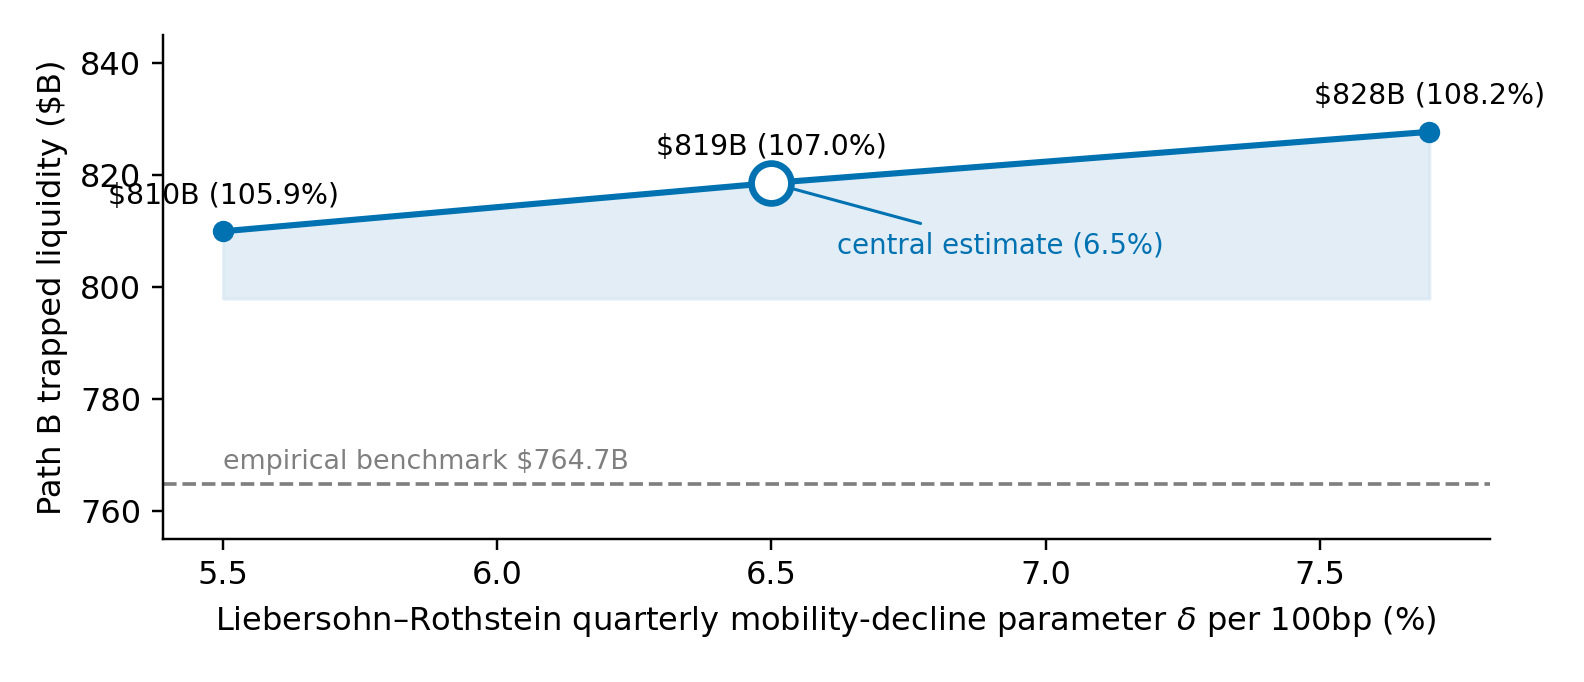
\includegraphics[width=0.80\textwidth]{fig6_elasticity_band}
\caption{Path~B recovery across the imported 5.5--7.7 percent mobility-response
band. The monotone relationship is a calibration sensitivity, not a sampling
confidence interval; the primary marginal additionally depends on the turnover
floor and the rule used to combine voluntary and involuntary prepayment.}
\label{fig:band}
\end{figure}

\begin{figure}[tbp]
\centering
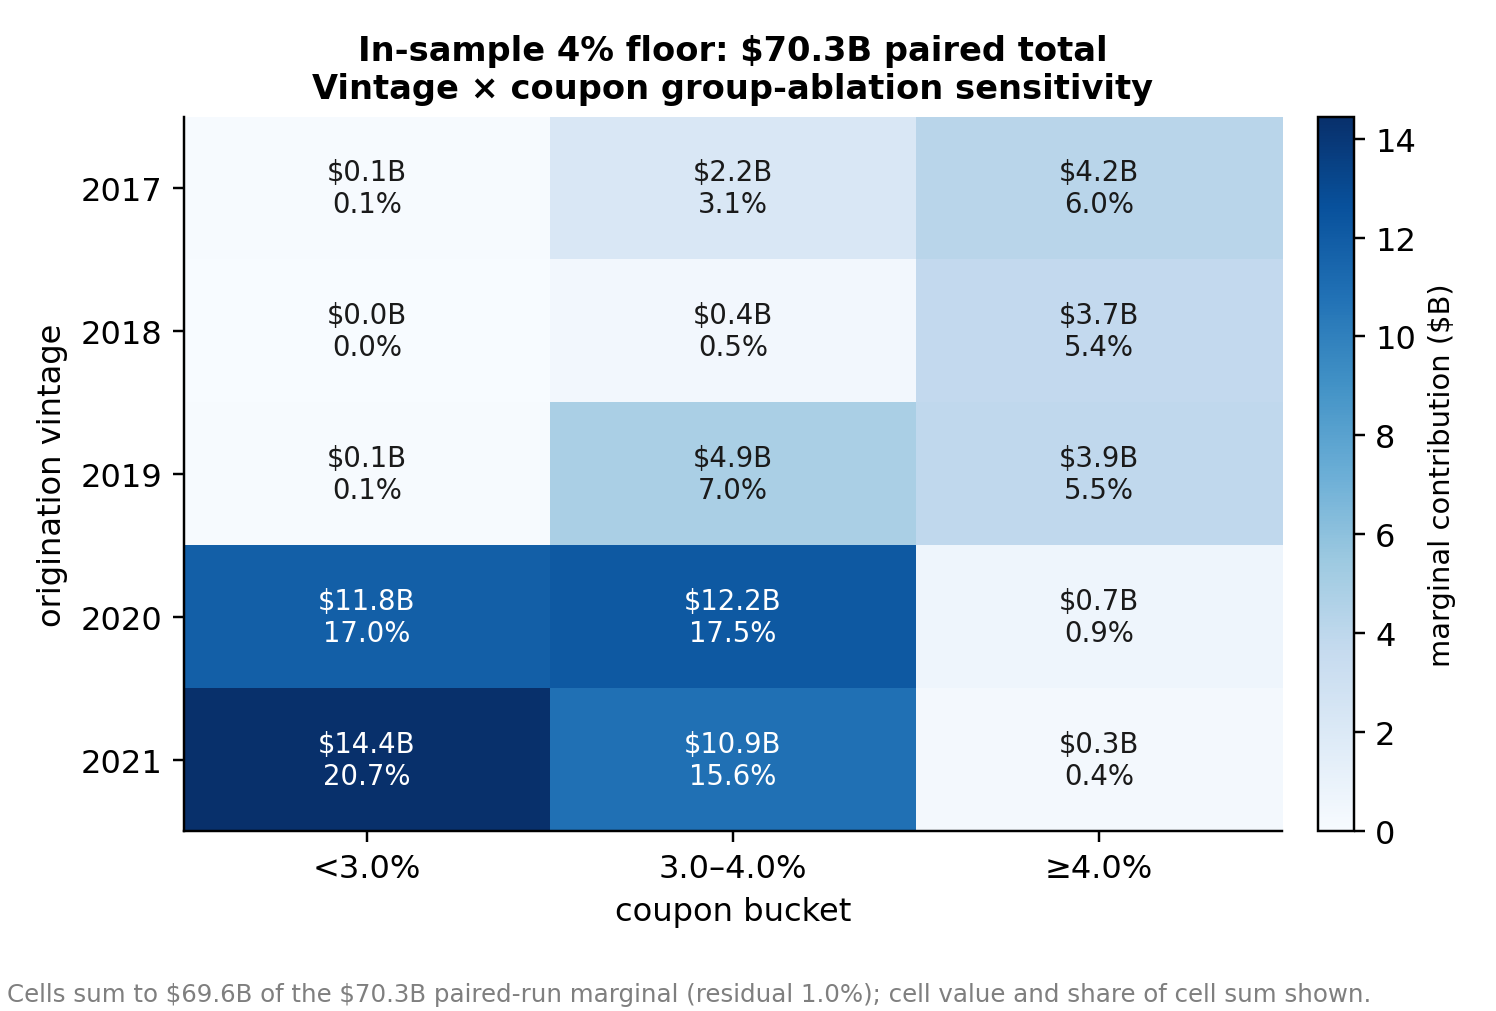
\includegraphics[width=0.76\textwidth]{fig11_marginal_decomposition}
\caption{Vintage-by-coupon contribution to the in-window lock-in marginal.
Every cell contributes positively, while no single cell dominates; the figure
supports a portfolio-wide composition reading rather than a representative-pool
interpretation.}
\label{fig:marginalcells}
\end{figure}

Six qualifications delimit the result. First, the exercise identifies a
model-based decomposition, not a causal effect; it uses no exogenous variation
in rate gaps. Second, the floor is estimated from realized behavior and sets
most of the aggregate level. Third, the response is imported from mobility and
applied to total prepayment. Fourth, the Freddie sample does not reproduce the
SOMA book's full agency, vintage, coupon, and term composition. Reweighting and
external-speed overlays bound that transport but do not eliminate it. Fifth, no
outcome-holdout months exist for the marginal, which is a difference between
simulations rather than an observed outcome. Sixth, the monthly path does not
validate the level: the simulated path trails the empirical path and does not
reproduce its timing after common trend removal.

\subsection{Validation and secondary estimators}\label{sec:pathb-fannie}

A matched Fannie Mae implementation returns a $+8.68$-point marginal. This is a
robustness check, not an outside test: it repeats the same functional form,
transported elasticity, and calibration logic on a second agency's loans, and
both agency samples omit important SOMA vintages. Its value is that the sign and
order of magnitude do not depend on Freddie alone.

\label{sec:patha}Path~A estimates a stratum-month Poisson prepayment hazard on the aggregated
Freddie universe and recovers 112.4\% of the shared-basis benchmark. It is
excluded from every headline range because its production specification lacks a
comparable propagated inferential object and its timing diagnostics do not
corroborate Path~B. I retain it as directional context only. Full
parameterization, delinquency transitions, floor inference, composition
diagnostics, Path~A estimation, and timing results are in the online appendix
and technical supplement.

\subsection{Interpretation}\label{sec:hazard-interp}

The hazard framework explains most of the cap-relative shortfall as an aggregate
level, but most of that level comes from scheduled amortization and the measured
turnover floor rather than the imported rate-gap response. The result therefore
does not say that lock-in caused 91.3\% of the shortfall. It says that the
rate-responsive increment lies within the disclosed ranges once the
rate-inelastic baseline is held fixed. That distinction separates the paper's
empirical claim from the larger institutional and household consequences
documented elsewhere.

\section{Discussion and Policy}\label{sec:discussion}
\subsection{Runoff composition and duration}\label{sec:discussion-fallout}

The decomposition changes how the cap-relative shortfall should be read. Slow
MBS runoff extended the duration of the Federal Reserve's holdings and left
more low-coupon mortgage duration with the public only gradually. It does not,
by itself, show that the Federal Reserve missed an aggregate balance-sheet
objective: Treasury runoff operated under separate caps, and this paper does
not estimate reserves or the aggregate securities path. The \$764.7 billion
benchmark measures the composition and timing of balance-sheet reduction, not a
failure to shrink the balance sheet.

The household and institutional effects are also not commensurable. Existing
work documents foregone moves and retained below-market financing value, while
this paper measures portfolio cash flow. The household estimate imported here
does not price search, housing supply, distribution, or general equilibrium.
Conversely, the cash-flow calculation does not value household mobility.
Statements about their relative importance are therefore directional, not a
ratio of comparable welfare quantities.

\subsection{Redemption-cap design}\label{sec:discussion-capdesign}

A passive-runoff cap can bind only if scheduled amortization and prepayment can
reach it. In this episode, scheduled principal plus the observed turnover floor
were below \$35 billion in essentially every month before adding the rate-gap
response. Because those components and a range for the response were observable
ex ante, the nonbindingness of the full cap was predictable as a band. The New
York Fed in fact projected monthly payments below the cap when the full ceiling
took effect \citep{nyfed2022}.

The design implication is not that the cap should have equaled realized runoff.
A cap also limits upside variation and communicates the maximum authorized pace.
It is that a policy document should separate the desired pace from a passive
cash-flow ceiling and publish the assumed amortization, turnover, and
rate-response inputs. If the desired pace exceeds that feasible band, the gap
must be closed by active sales, reinvestment changes, or another instrument
rather than by a higher passive cap. Detailed monthly and state-contingent grids
are in the technical supplement.

\subsection{The Danish market-value-repurchase counterfactual}\label{sec:discussion-policy}\label{sec:abm-danish}

The U.S. mortgage contract requires payoff at face value when a borrower sells
or refinances. Danish borrowers may instead purchase the bonds funding their
mortgage at market value and deliver them to the mortgage bank. When rates rise,
the bond price falls, offsetting part of the cost of giving up a low coupon.
The counterfactual changes the payoff rule while retaining the SOMA portfolio
and the hazard machinery.

The preferred rule-only transplant anchors Danish mobility at the estimated
U.S. zero-gap hazard and imports the flatter Danish rate response from
\citet{berger2026}. Under face accounting, the Danish leg produces a
+\$61.2 billion U.S.-minus-Danish gap at zero refinance-in-place, rising to
+\$256.8 billion across the reported refinancing sweep. The positive sign is
forced by the shared zero-gap anchor, so the informative result is its
magnitude. A bracketing case that also imports the lower Danish mobility level
reverses the gap to -\$99.9 billion. Cash accounting at the re-derived bond
discount reverses the preferred-anchor result to -\$51.0 billion, and product
composition can reverse it as well. The counterfactual is therefore anchor-,
incidence-, and product-mix-dependent.

\begin{table}[H]
\centering
\small
\caption{Danish counterfactual: anchor and accounting determine the sign.}
\label{tab:danish-compact}
\begin{threeparttable}
\begin{tabular}{@{}p{4.0cm}p{3.4cm}p{2.5cm}p{4.0cm}@{}}
\toprule
Counterfactual & Accounting or level anchor & U.S.--Danish gap & What changes \\
\midrule
Rule-only transplant & Face accounting & $+\$61.2$ billion & U.S. zero-gap intercept; zero refinance-in-place edge \\
Rule-only transplant & Cash accounting & $-\$51.0$ billion & Same face retirement, but bought-back face credited at its re-derived market value \\
Rule plus Danish mobility level & Face accounting & $-\$99.9$ billion & Imports Denmark's descriptive moving level as well as the flatter response \\
\bottomrule
\end{tabular}
\begin{tablenotes}[flushleft]\footnotesize
\item Notes: Gap is U.S. trapped liquidity minus Danish trapped liquidity. The first row is benchmark-consistent because the SOMA benchmark and runoff caps are face-denominated. The cash row answers the distinct reserves-drained question. These rows are alternative readings, not additive effects. The face gap also reverses when the Danish interest-only share exceeds 34.3\%. None prices TBA liquidity, transition, tax, servicing, or general-equilibrium costs.
\end{tablenotes}
\end{threeparttable}
\end{table}

This exercise does not price a U.S. transition to the Danish structure.
Market-value repurchase requires liquid trading in the specific funding bonds,
whereas the U.S. TBA market derives liquidity from standardized, fungible pools.
The loss of that liquidity, investor compensation, tax treatment, servicing,
and distributional effects are outside the calculation. The result establishes
that the face-value payoff rule affects cash-flow incidence; it does not
establish that adopting the Danish system would raise welfare. Full discount,
incidence, product-mix, and fine-grid mechanics are preserved in the technical
supplement.

\section{Robustness Checks}\label{sec:robustness}
The robustness exercises answer whether the main interpretation changes when
the floor, functional form, population, accounting, or estimator changes. Full
grids and diagnostics are in the online appendix and technical supplement.

\subsection{Floor and functional form}\label{sec:robustness-floor}

At the central elasticity, the defensible off-window floor range produces
$+4.3$ to $+6.8$ points under the production maximum form. Propagating
sampling error gives the binding $[+1.9,+9.1]$ interval. The additive
competing-risks form moves the level sharply but leaves the marginal near
$+11.2$ points across 3--5\% floors. The form-conditional hull is $+3.5$ to
$+13.1$. Seasonal and cyclical variants largely measure dispersion induced by
the maximum rather than timing; their small order component does not credential
the monthly path. These checks preserve a positive marginal but rule out a
single model-free magnitude.

\begin{table}[H]
\centering
\small
\caption{Uncertainty and robustness for the Path~B lock-in marginal.}
\label{tab:uncertainty-compact}
\begin{threeparttable}
\begin{tabular}{@{}p{4.3cm}p{3.4cm}p{6.0cm}@{}}
\toprule
Dimension & Reported range & Meaning \\
\midrule
Floor-read sampling uncertainty & $[+1.9,+9.1]$ pp & Restricted wild-cluster inversion on 31 strata, propagated through the frozen floor-to-marginal map at the central elasticity; binding coverage-bearing interval \\
Elasticity calibration range & $+3.9$ to $+7.5$ pp & Published 5.5--7.7\% mobility-response band crossed with the clean off-window floor range; no coverage interpretation \\
Functional-form range & $+3.5$ to $+13.1$ pp & Reported hull across maximum/additive floor combinations and the disclosed transform checks; a specification range, not a confidence interval \\
Full calibration box & $+2.1$ to $+13.2$ pp & Floors 2--6\% crossed with the 5.5--7.7\% band under the production maximum form; no coverage interpretation \\
\bottomrule
\end{tabular}
\begin{tablenotes}[flushleft]\footnotesize
\item Notes: The $[+1.9,+9.1]$ interval prices sampling error in the off-window floor read only. It is not an interval for the transported elasticity and does not absorb functional-form uncertainty. The additive-form marginal is approximately $+11.2$ points across 3--5\% floors.
\end{tablenotes}
\end{threeparttable}
\end{table}

\subsection{Population and cross-design checks}\label{sec:robustness-crossdesign}\label{sec:robustness-hybrid}

Reweighting the hazard simulation to the SOMA coupon composition changes the
aggregate level but not the qualitative decomposition. Agency, vintage, and
term mismatches remain because neither loan sample spans the whole SOMA book.
The Fannie reproduction returns a similar marginal, while the Ginnie speed
overlay and observed-vintage bound leave the conventional-loan result positive.
These are transport checks rather than external identification.

The paired ABM exercise is deliberately adverse to a simple paradigm story.
Real structural covariates raise the recalibrated ABM above its pre-committed
50\% threshold, and book reweighting raises it further. Conversely, the hazard
structure recovers a similar level on a synthetic population. The first result
shows that the ABM level depends materially on population and calibration; the
second shows that the hazard level is carried substantially by its calibrated
structure. Together they withdraw, rather than establish, the claim that the
original ABM--hazard gap isolates modeling paradigm.

\subsection{Benchmark and secondary checks}\label{sec:robustness-benchmark}\label{sec:robustness-scale}\label{sec:robustness-synthesis}

Settlement-aware allocation changes the expectations-based complement but not
the cap-relative benchmark. Alternative settlement kernels, curtailment
profiles, and accounting bases move levels while common adjustments cancel
from paired marginals. Increasing the ABM population reduces seed dispersion
without closing its level or path mismatch. Path~A remains directional context,
not a corroborating estimate. None of these checks supplies the exogenous
variation required for a causal lock-in estimate.

The robustness conclusion is therefore bounded. The positive rate-responsive
increment survives every reported floor anchor and the second-agency
reproduction. Its magnitude remains conditional on the floor, combination
rule, transported elasticity, and sample-to-book mapping. That is why the paper
reports ranges and keeps the aggregate level distinct from the marginal.

\section{Conclusion}\label{sec:conclusion}
The Federal Reserve's agency-MBS runoff fell \$764.7 billion below its phased
QT caps through November 2025, but that gap was not a direct measure of mortgage
lock-in. Under the production hazard form, scheduled amortization and a turnover
floor measured from realized deep-discount cohorts recover 85.7\% of the
benchmark even after the imported rate response is switched off. Adding that
response raises recovery to 91.3\%. The paper therefore identifies a bounded
marginal over a rate-inelastic null, not the full level: $[+1.9,+9.1]$
percentage points when the off-window floor's sampling error is propagated,
with additional form and calibration ranges stated separately.

The result has a direct cap-design implication. Passive runoff ceilings should
be evaluated against ex-ante ranges for scheduled amortization, baseline
turnover, and rate-responsive prepayment. Here those inputs implied that the
\$35 billion monthly MBS ceiling would rarely bind. A Danish-style
market-value-repurchase rule changes the cash-flow incidence of lock-in, but
its U.S. counterfactual changes sign across defensible level and accounting
anchors and does not price the TBA liquidity cost of institutional redesign.

\subsection{Limitations and future work}\label{sec:limitations}

The decomposition is model-based rather than causal: it uses no exogenous
variation in rate gaps. Its elasticity is imported from mobility estimates and
mapped to total prepayment. Its turnover floor mixes discretionary,
refinancing, and involuntary exits and is measured from realized behavior. The
Freddie and Fannie samples do not reproduce the SOMA book's complete agency,
vintage, coupon, and term composition. No outcome-holdout months validate the
simulated marginal, and no estimator reproduces the monthly path after common
trend removal. The ABM comparison remains confounded by population and
calibration, while the Danish exercise leaves transition costs, investor
pricing, tax, servicing, and distributional effects unmeasured.

These limitations define the next empirical work: identify the mobility and
refinancing components separately, estimate the response with plausibly
exogenous rate-gap variation, extend coverage to the missing SOMA vintages and
agencies, and price contract redesign jointly for households and MBS investors.
They do not overturn the narrower conclusion supported here: most of the
cap-relative shortfall is reproduced by rate-insensitive cash flows, while the
increment associated with the transported lock-in response is positive and
material but bounded.

\clearpage
\bibliographystyle{plainnat}
\bibliography{references}

\clearpage
\appendix

\noindent\textbf{Online Appendix.} The appendices that follow are for online publication. The run ledger of superseded figures and the pre-committed-rule adjudication record form a standalone document in the replication package (\texttt{replication\_appendices}). Its cross-references resolve against this manuscript.

\section{Accounting benchmark and sample construction}\label{app:benchmark}

The benchmark is the cumulative shortfall of realized SOMA agency-MBS runoff
relative to the announced cap over the active QT window. Holdings are aligned to
month end, scheduled principal is separated from unscheduled principal, and
negative implied prepayment is clipped at zero. The resulting shortfall is
\$764.7 billion. This is an accounting object, not an estimate of causal lock-in:
issuance composition, servicing, reporting dates, and other market frictions can
also affect runoff. Four exact-zero implied-prepayment months arise when reported
runoff falls below the scheduled-amortization floor; consequently the paper makes
no monthly-timing claim.

The hazard panel uses agency mortgage cohorts linked to note-rate gaps and loan
characteristics. Path~B draws 75{,}000 loans from the Freddie Mac 2017--2021
conventional 30-year origination universe; 40{,}234 remain active when QT opens,
and the production calculation evaluates 1{,}683{,}124 active loan-months.
Fifteen-year securities remain in the SOMA accounting benchmark but not this
loan-level hazard sample. The sample also omits Ginnie collateral and vintages
outside 2017--2021. On the book's agency-by-vintage joint cells, the sampled
conventional-and-in-window intersection is 51.0\% of SOMA face (51.8\% upper
bound from cell truncation), not the 66.2\% vintage-only marginal. Published
speed overlays bound the Ginnie exclusion at \$20--\$47 billion and observed
out-of-window vintage speeds imply an \$11.7 billion bound, both signed toward
the unadjusted simulation overstating trapped liquidity. These are external
bounds, not structural inclusion of the missing loans.

The matched Fannie Mae reproduction is a robustness check, not an outside test.
It applies the same transported elasticity, maximum-floor form, and calibration
logic to a second agency sample and returns a $+8.68$-point marginal. Both agency
samples share the policy window and omit parts of the SOMA vintage support, so
the result checks agency dependence without supplying independent identification.

\section{Hazard estimand and parameterization}\label{app:params}

For loan $i$ in month $t$, the production prepayment and default hazards are
\begin{align}
h^{\mathrm{prep}}_{i,t}
 &= \max\!\left\{\underline h,
 h_0(a_{i,t})\exp\!\left(\beta_1 g_{i,t}+\beta_Fz_i^{\mathrm{FICO}}
 +\beta_Lz_i^{\mathrm{LTV}}+\beta_BB_{s(i),t}\right)\right\},
 \label{eq:appendix-prep}\\
h^{\mathrm{def}}_{i,t}
 &=h^{\mathrm{def}}_0\exp\!\left(\gamma_r\sigma_{i,t}
 +\gamma_Fz_i^{\mathrm{FICO}}+\gamma_Lz_i^{\mathrm{LTV}}\right),
 \quad \sigma_{i,t}=\max\{0,-\widetilde g_{i,t}\}.
 \label{eq:appendix-default}
\end{align}
Here $g_{i,t}$ is coupon minus the prevailing mortgage rate in 100-basis-point
units, negative when the loan is locked in, and $\widetilde g_{i,t}=g_{i,t}/100$
is its decimal form in the default equation. The baseline $h_0(a)$ follows the
100-PSA seasoning ramp. The floor $\underline h$ is the SMM equivalent of the
stated annual CPR. Burnout $B_{s(i),t}$ is the stratum's cumulative prepaid UPB
share since the QT opening; it is initialized at zero and capped at one.
Competing exits are applied monthly to surviving balances, followed by scheduled
amortization at each loan's note rate and aggregation to the SOMA balance path.

\begin{table}[tbp]
\centering
\small
\caption{Key Path~B parameters and accounting conventions.}
\label{tab:pathb-parameters-compact}
\begin{tabular}{@{}p{3.5cm}p{3.0cm}p{7.0cm}@{}}
\toprule
Object & Production value & Role and provenance \\
\midrule
Mobility response $\delta$ & 6.5\%; band 5.5--7.7\% & Imported quarterly proportional decline per 100 bp; converted by the survival transform to $\beta_1=0.0686$ \\
Turnover floor $\underline h$ & 4\% annual CPR in-sample; 4.695--5.334\% off-window & Deep-discount realized turnover; includes discretionary and involuntary exits \\
Seasoning baseline & 100 PSA & CPR ramps by 0.2 points per month to 6\% at month 30 \\
Burnout coefficient $\beta_B$ & $-0.5$ & Cohort-level cumulative-prepayment state \\
Default baseline $h^{\mathrm{def}}_0$ & $3\times10^{-4}$ monthly & Competing default prior; approximately 0.36\% annually \\
Shared accounting & common \$69.6 billion curtailment netting & Applied identically to central and null legs, so it cancels from the marginal \\
\bottomrule
\end{tabular}
\end{table}

The central leg uses the transported $\beta_1$; the rate-inelastic null sets
$\beta_1=0$ while holding the floor, PSA baseline, burnout, covariates, default,
loan population, randomization, amortization, and accounting layer fixed. The
central-minus-null difference is therefore the paper's model-based lock-in
marginal. At the off-window midpoint the central level is 91.3\% of the
benchmark and the null is 85.7\%; these are percentages, not dollar amounts.
The binding $[+1.9,+9.1]$-point interval propagates sampling error in the floor
read at the central elasticity only. Calibration and form ranges are reported
separately in Table~\ref{tab:uncertainty-compact}.

\section{ABM mechanics and diagnostic role}\label{sec:method-abm}
\label{sec:method-frictions}\label{app:abmspec}

The agent-based model simulates 10{,}000 heterogeneous households. Coupons and
origination dates are drawn from the live CUSIP-level SOMA composition; income,
home value, age, and mortgage balance are calibrated from aggregate series. A
move compares the current payment with the payment on the outstanding balance
refinanced at the market rate over a fresh original term. The decision rule also
contains moving and closing costs, housing-search and sentiment frictions, a
43\% payment-to-income screen, 2.25-times loss aversion on payment increases,
and an author-calibrated wait-and-see freeze. Approved movers prepay; balances
then receive scheduled amortization and common curtailment before the simulated
roll-off is scored against the phased cap. The mobility scale is recalibrated to
reproduce 4--5\% deeply out-of-the-money turnover, so matching that floor is an
input rather than evidence for the model.

The U.S. rule requires payoff at par. The Danish counterfactual permits
market-value repurchase, but the production exercise anchors the moving hazard
to external Danish evidence rather than allowing the pricing proxy to determine
it. The ABM recovers only 10--17 percent of the benchmark across its production
variants, overpredicts average CPR, and fails to match monthly shape. It is used
as a mechanism stress test and not averaged with the hazard estimate. Its
real-covariate variant reaches 59.3\% after recalibration and 76.3\% after book
reweighting, crossing the pre-committed threshold that withdraws the former
modeling-paradigm interpretation. No ABM marginal is reported because its two
plausible nulls disagree even in sign. Full utility equations, parameter
provenance, interpolation checks, Monte Carlo dispersion, and failed variants
remain in the technical supplement.

\section{Composition and policy mappings}\label{app:composition}

The SOMA portfolio is concentrated in low-coupon 30-year pools: the parsed
weighted-average coupon is about 2.55 percent, with the 2.0 and 2.5 percent
buckets accounting for roughly 69 percent of 30-year face value. That composition
widens the gap to prevailing mortgage rates and explains why representative-loan
examples are not sufficient. Results are aggregated on declining balances, so
counterfactual payoff in one month reduces the exposure available thereafter.

The Danish policy exercise is a mechanism comparison, not a welfare calculation.
Using the preferred external anchor, Danish-style market-value repurchase changes
runoff by \$61.2 billion relative to the zero-refinancing benchmark; the full
parameter sweep spans a much wider range. A Danish-level hazard maps to
$-\$99.9$ billion and a cash-purchase window to a \$51.0 billion reduction under their
stated counterfactual baselines. These quantities are not mutually additive and
do not price implementation costs, TBA-market effects, redistribution, or
general-equilibrium responses.

\section{Floor, form, and timing robustness}\label{app:floormech}
\label{sec:robustness-extensions}\label{sec:robustness-wal}
\label{sec:robustness-pipeline}\label{sec:robustness-seasonalfloor}

The main identifying uncertainty is how voluntary and involuntary prepayment
combine. Under the preferred maximum rule, dispersion in the floor creates a
one-sided Jensen effect: high floor realizations bind, while low realizations are
truncated where voluntary hazard is already larger. Seasonal and cyclical-floor
experiments therefore mostly measure floor dispersion rather than calendar
timing. Holding the floor's exposure-weighted mean at 4 percent changes the
marginal by \$4.9 billion, at most 7 percent of the in-sample marginal. Permuting
the same monthly floor values preserves 89.2 percent of that movement on average.

\begin{table}[tbp]
\centering
\small
\caption{Central off-window floor-by-elasticity grid: lock-in marginal (percentage points of the \$764.7 billion benchmark).}
\label{tab:floor-elasticity-grid}
\begin{threeparttable}
\begin{tabular}{@{}lrrr@{}}
\toprule
Annual turnover floor & 5.5\% response & 6.5\% response & 7.7\% response \\
\midrule
4.695\% & $+6.08$ & $+6.77$ & $+7.46$ \\
4.991\% & $+5.04$ & $+5.57$ & $+6.09$ \\
5.334\% & $+3.89$ & $+4.27$ & $+4.62$ \\
\bottomrule
\end{tabular}
\begin{tablenotes}[flushleft]\footnotesize
\item Notes: The rows are the clean pre-episode 2018 floor reads; columns sweep the published mobility-response calibration band. The grid is monotone by construction and has no coverage interpretation. Its central cell rounds to the $+5.6$-point, \$42.6 billion anchor. Sampling uncertainty in the floor read is propagated separately.
\end{tablenotes}
\end{threeparttable}
\end{table}

\begin{table}[tbp]
\centering
\small
\caption{Functional-form comparison at the central 6.5\% response.}
\label{tab:floor-form-compact}
\begin{threeparttable}
\begin{tabular}{@{}lrrr@{}}
\toprule
Combination rule & 3\% floor & 4\% floor & 5\% floor \\
\midrule
Maximum & $+10.82$ & $+9.20$ & $+5.54$ \\
Additive competing risks & $+11.29$ & $+11.25$ & $+11.21$ \\
\bottomrule
\end{tabular}
\begin{tablenotes}[flushleft]\footnotesize
\item Notes: Under the maximum, a higher floor censors more of the rate response. Under $1-(1-h_{\rm floor})(1-h_{\rm voluntary})$, the marginal is almost floor-invariant but both central and null levels change sharply. These are alternative specifications, not confidence intervals.
\end{tablenotes}
\end{threeparttable}
\end{table}

The pre-committed timing criterion is formally met by some seasonal variants, but
it is also met by wrong-month rotations, scrambled calendars, and a
zero-elasticity null. The result has no discriminatory power. All conclusions are
therefore restricted to cumulative levels. Alternative turnover-floor levels,
the competing-risks form, the 15-year fold-in, duration calculations, and the
rate-gap unit audit are reported as separate specification checks; they are not
folded into the floor-read sampling interval. None overturns the conclusion that
lock-in is economically present but explains only a minority of the accounting
shortfall.

\section{Excluded design and replication record}\label{app:patha-detail}
\label{app:ridge}\label{app:theil}

Path~A is excluded from every headline range. It estimates aggregate timing relationships between market rates, refinancing
conditions, and SOMA runoff. Its results are retained for transparency, including
ridge stabilization and dynamic-fit decompositions, but are not used in the
headline because the short window, common trends, weak effective support, and
sensitivity to timing conventions prevent a defensible causal interpretation.
Every superseded number, figure, diagnostic, and parameter-level derivation is
available in the standalone technical replication supplement, which embeds the
complete 147-page pre-compression manuscript. This online appendix is limited to
the material needed to interpret and reproduce the publication-facing claims.

\end{document}
